\documentclass[14pt,a4paper]{article}

\usepackage{amsmath}
\usepackage{amssymb}

\usepackage[T2A]{fontenc}
\usepackage[utf8]{inputenc}
\usepackage[russian]{babel}

\usepackage{graphicx}
\graphicspath{ {./materials/} }
\usepackage[font=bf]{caption}

\title{Задачи по байесовскому подходу к классификации}
\author{Денисов Д.М.}
\date{}

\begin{document}
    \maketitle

    Исходные данные:
    \[
        \begin{gathered}
            p(x | y = -1) = \frac{1}{\pi (1 + x^2)} \sim Cauchy(0, 1), \\
            p(x | y = +1) = \frac{1}{3} I_{[a, b]} \sim U(0, 3), \\
            \lambda_{-} = 2, \ \lambda_{+} = 1, \\
            p(y = -1) =  0.4, \ p(y = +1) = 0.6.
        \end{gathered}
    \]

    \section{Оптимальный байесовский классификатор}

    Имеем:
    \[
        \begin{aligned}
            a^*(x) &= \underset{y}{\arg\!\max} \ \lambda_y P(y) p(x | y) \\
            &= \underset{y}{\arg\!\max} \ \left\{ \lambda_{-} P(y = -1) p(x | y = -1), \lambda_{+} P(y = +1) p(x | y = +1) \right\} \\
            &= \underset{y}{\arg\!\max} \ \left\{ \frac{0.8}{\pi (1 + x^2)}, 0.2 I_{[a, b]} \right\} \\
            &= \underset{y}{\arg\!\max} \ \left\{ f(x), g(x) \right\}.
        \end{aligned}
    \]

    Графики распределений $f(x)$ и $g(x)$ представлены на рис. \ref{fig:distribs}.
    \begin{figure}[h]
        \centering
        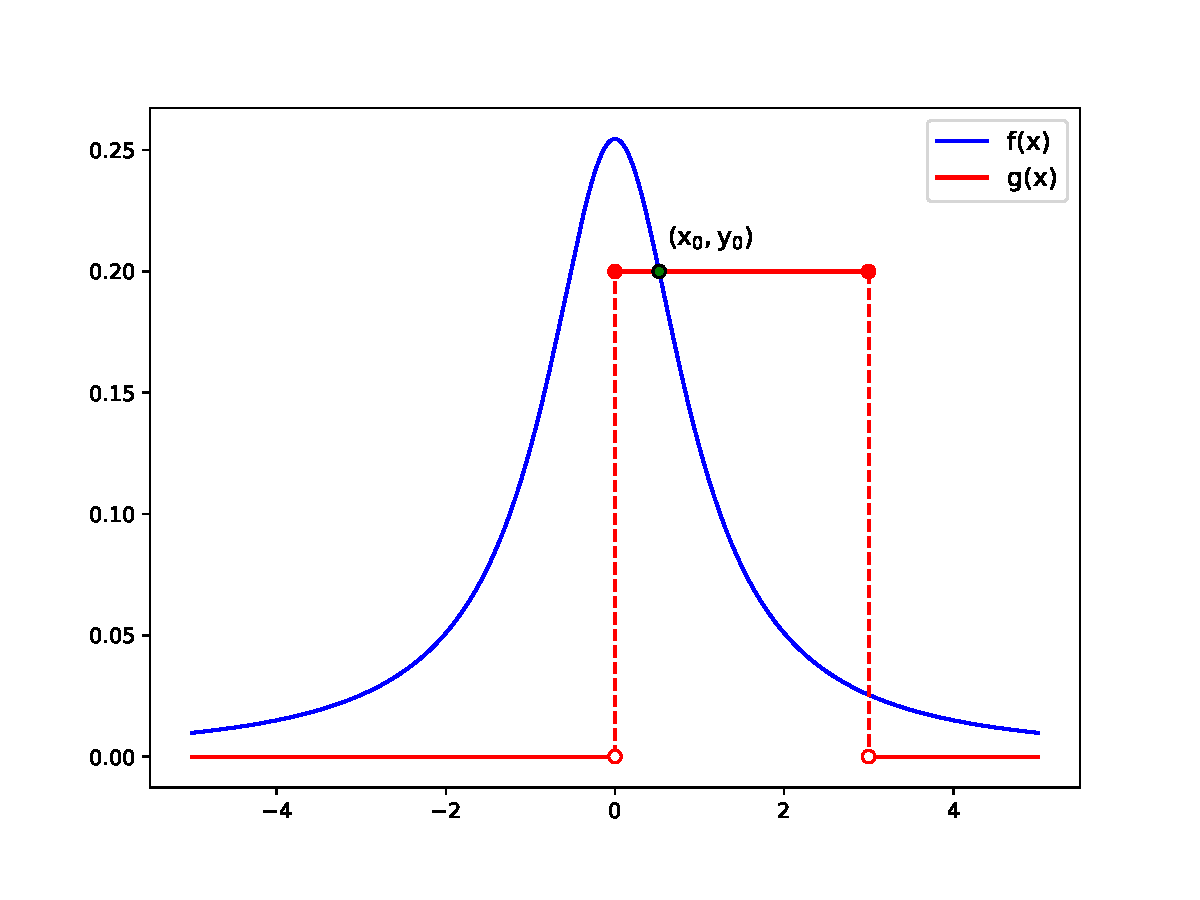
\includegraphics[width=\textwidth]{distribs.pdf}
        \caption{Графики распределений}
        \label{fig:distribs}
    \end{figure}

	Из рис. \ref{fig:distribs} видно, что
	\[
		g(x) \geq f(x) \iff x \in [x_0, 3].
	\]
	
	Таким образом, оптимальный классификатор будет иметь вид
	\[
		a^*(x) = \left\{
		\begin{aligned}
			& -1, \ x \in (-\infty, x_0) \cup (3, +\infty) \\
			& +1, \ x \in [x_0, 3]
		\end{aligned}
		\right..
	\]
	
	Координату $x_0$ найдём следующим образом:
	\[
	\begin{gathered}
		f(x_0) = g(x_0) = 0.2 \implies \frac{0.8}{\pi (1 + {x_0}^2)} = 0.2 \implies \\
		\implies \pi (1 + {x_0}^2) = 4 \implies x_0 = \sqrt{\frac{4}{\pi} - 1}.
	\end{gathered}
	\]
	
    \section{Оптимальный средний риск}
    Имеем:
    \[
    	\begin{aligned}
    		R^* &= \iint L(a^*(x), y) p(x, y) \,dx\,dy \\
    		&= \iint \lambda_y [a^*(x) \neq y] p(x | y) P(y) \,dx\,dy \\
    		&= \iint \lambda_y (1 - [a^*(x) = y]) p(x | y) P(y) \,dx\,dy \\
    		&= \int \underset{y}{\min} \ \lambda_y p(x | y) P(y) \,dx\,dy \\
    		&= \int \underset{y}{\min} \ \{ \lambda_{-} p(x | y = -1) P(y = -1), \lambda_{+} p(x | y = +1) P(y = +1) \} \,dx\,dy \\
    		&= \int \underset{y}{\min} \ \{ f(x), g(x) \} \,dx\,dy.
    	\end{aligned}
    \]
    
    Аналогично пункту 1, получаем:
    \[
    	\begin{aligned}
    		R^* &= \int_{-\infty}^{x_0} g(x) \,dx + \int_{x_0}^{3} f(x) \,dx + \int_{3}^{+\infty} g(x) \,dx \\
    		&= \int_{0}^{x_0} 0.2 \,dx + \int_{x_0}^{3} \frac{0.8}{\pi (1 + x^2)} \,dx \\
    		&= 0.2 x_0 + \frac{0.8}{\pi} (\arctan{3} - \arctan{x_0}) \approx 0.299958 \approx 0.3.
    	\end{aligned}
    \]

    \section{Наивный байесовский классификатор}
    Найдём наивный байесовский классификатор так:
\end{document}